% !TeX spellcheck = en_US
\section{Trajectory Optimization}
\label{sec:trajectory-optimization}

    Trajectory optimization is a method for designing the motion of a system to achieve a desired goal. It involves the calculation of an optimal path taking  various constraints and objectives into account. The term trajectory refers to the path an agent travels as a function of time. The term trajectory optimization is therefore the set of methods used to obtain the best trajectory, usually by selecting appropriate inputs to the system,~\ie controls, as functions of time. The comprehensive policy of optimization is to minimize the objective function subject to a number of constraints and restrictions.~\cite{Kelly2017} In the course of this work a trajectory optimization was performed via finding a minimum of constrained nonlinear multivariable functions.\\ % Therefore, the comprehensive policy is to minimize the objective function subject to the system dynamics and constraints.

    The process typically involves the following steps~\cite{Kelly2017}:
    \begin{enumerate}
        \item Modeling the robot's dynamics: A mathematical model of the robot's movement is created, which takes into account the robot's kinematics, dynamics, and control inputs.
        \item Specifying the constraints: The constraints that must be satisfied by the robot's motion are defined, such as bounds on the joint angles and torques, as well as collision avoidance constraints.
        \item Defining the objective: The objective function to be optimized is defined, which might include a trade-off between energy efficiency, speed, and smoothness of the motion.
        \item Solving the optimization problem: An optimization algorithm is applied to find the path that minimizes the objective function while satisfying the constraints.
        \item Generating the motion trajectory: The optimal path is transformed into a set of points that define the motion trajectory for the robot.
    \end{enumerate}
    
    The following sections describe the individual steps that were carried out in more detail.

        \subsection*{Assumptions}
        
        Within this work it is assumed that the trajectory is single-phase and of continuous time, meaning the system dynamics are continuous throughout the entire trajectory. The dynamics, the objective, and the constraints are smooth, consistent and potentially non-linear. Furthermore, the robot is considered to be left-right symmetric, allowing to search for a periodic walking gait with a single step instead of a stride. A periodic gait requires that the joint trajectories, consisting of the joint angles, their rates, and the associated torques, are the same for each successive step.~\cite{Kelly2017}
        
        \subsection*{Constraints}
        
        % The optimization problem is subject to a number of constraints and restrictions. 
        The first and possibly most important constraint is the system dynamics. In addition, limits are defined for the boundary condition, restricting the initial and final states of the system, including upper and lower limits for the joint angles and joint velocities. Furthermore, the initial state is limited to the~\glsxtrshort{vlo}$_0$,~\ie the stance leg always starts vertically. % Further path constraints were used to keep the foot of the robot above the ground, for example
        
        % The optimization is subject to a variety of limits and constraints. The first, and perhaps most important, of these constraints is the system dynamics. Next is the path constraint, which enforces restrictions along the trajectory. A path constraint could be used, for example, to keep the foot of a walking robot above the ground during a step. Another important type of constraint is a nonlinear boundary constraint, which puts restrictions on the initial and final states of the system. Such a constraint would be used, for example, to ensure that the gait of a walking robot is periodic.
        
        % \subsection{Transcription}

        %     The key feature of a direct method is that it discretizes the trajectory
        %     optimization problem itself, typically converting the original trajectory optimization problem into a nonlinear program.

        %     transform trajectory optimization problem into constrained parameter optimization (NLP)

        \subsection*{Nonlinear Programming}
        
        Most direct collocation methods transform a continuous-time trajectory optimization problem into a~\glsxtrfull{nlp},~\ie a constrained parameter optimization problem that has nonlinear terms in either its objective or its constraint function. This nonlinearity makes~\glsxtrshort{nlp} problems more difficult to solve, as the objective function and/or constraints can have multiple local minima (or maxima) and the global minimum (or maximum) may not be easily accessible.~\cite{Kelly2017} A common formulation for a nonlinear program is as follows:
        
        \begin{align}
            \begin{array}{ll}
                \min\limits_{\boldsymbol{a}}     & f(\boldsymbol{a}) \\
                \text{subject to }  & h(\boldsymbol{a}) = 0 \\
                                    & g(\boldsymbol{a}) \leq 0, \\
                                    & \boldsymbol{a}_{lb} \leq \boldsymbol{a} \leq \boldsymbol{a}_{ub}
            \end{array}
        \end{align}
        % \noindent
        
        where$~\boldsymbol{a}$ denotes the vector of design variables,$~f(\boldsymbol{a})$ the objective function,$~h(\boldsymbol{a})$ the equality constraint functions,$~g(\boldsymbol{a})$ the inequality constraint functions and$~\boldsymbol{a}_{lb},~\boldsymbol{a}_{ub}$ the lower and upper bounds, respectively.
        
        \subsection*{System Dynamics}
        
        During single support (see figure~\ref{fig:vlo}), the system has six~\glsxtrfull{dof}: the absolute angles of both lower legs, \ie of the knee joints ($q_5$ and $q_7$), both upper legs, \ie of the hip joints ($q_4$ and $q_6$), the torso ($q_3$) as well as the vertical displacement, which depends on the springs mounted inline to the legs ($q_2$). The~\glsxtrshort{dof} can be seen in figure~\ref{fig:jenafox-dof}. Hereafter, the~\glsxtrshort{dof} of the system are cumulated into the single vector$~\gls{q}$. Since it is a second order dynamical system, the derivative of the configuration, $\dot{\gls{q}}$ must also be included. Thus, the state can be described with$~\begin{bmatrix} \gls{q} & \dot{\gls{q}} \end{bmatrix}^\textrm{T}$ and the dynamics as$~\begin{bmatrix} \dot{\gls{q}} & \ddot{\gls{q}} \end{bmatrix}^\textrm{T}$, where $\gls{q}$ are the angles,$~\dot{\gls{q}}$ the angular rates and$~\ddot{\gls{q}}$ the accelerations, respectively. Since the initial and final states of the optimization problem are defined using the~\glsxtrshort{vlo}, the start and end position of the stance leg is always vertically. Thus, the respective hip and knee angles as well as the corresponding angular velocities can be neglected. This results in six parameters which have to be considered: The hip and knee angles of the swing leg, the angle of the upper body and their angular velocities. Furthermore, to obtain a variation of the velocity vector,$~\gls{lambda}$,~\ie the angle of~\gls{v}$_{\glsxtrshort{com}}$, is also included. Table~\ref{tab:initial-conditions} shows the initial condition used in the multi-body simulation.
        
        \begin{figure}[htb]%
            \centering%
            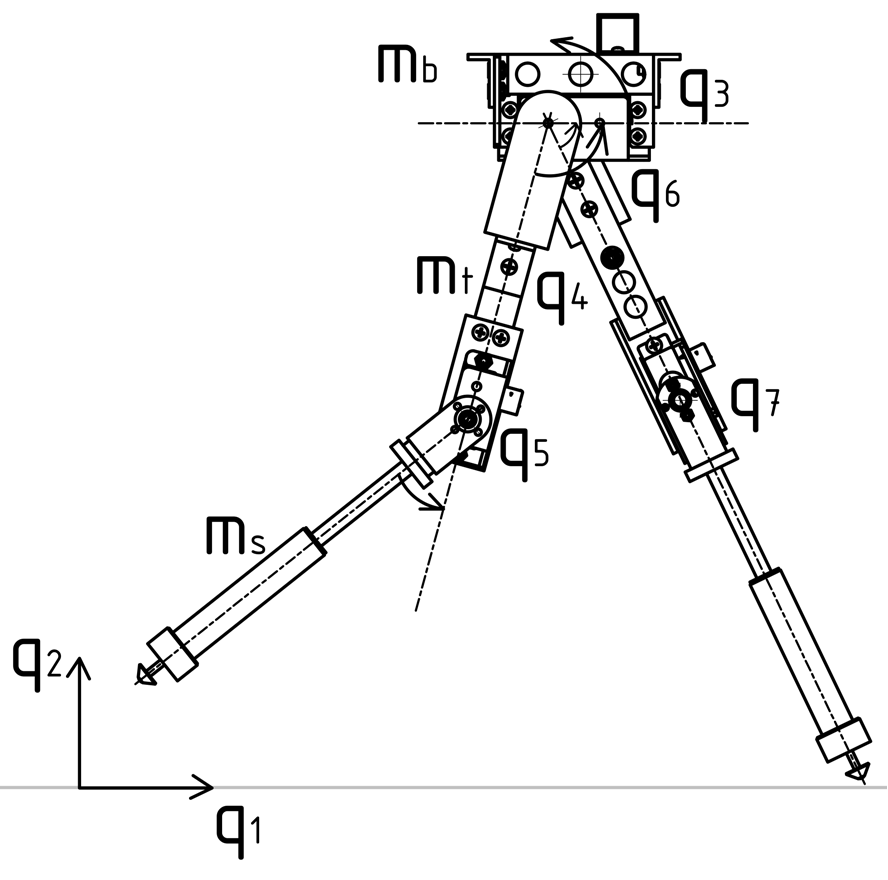
\includegraphics[width=0.8\linewidth]{jenafox/basic-coordinates/basic-coordinates.png}
            \caption{Degrees of freedom of the basic mechanical setup. The trunk (mass $m_b$) has three degrees of freedom ($q_1,~q_2,~q_3$), hip and knee of the right leg connect the thigh ($m_t$) to the body and shank ($m_s$) to the thigh respectively by one degree of freedom each ($q_4,~q_5$), the same counts for the left side ($q_6,~q_7$). (Adapted from~\cite{Renjewski2013}, p. 37)}%
            \label{fig:jenafox-dof}%
        \end{figure}
        % \noindent

        \begin{table}[H]
            \caption{Initial conditions used in the multi-body simulation consisting of the knee and hip angles of the swing leg,$~q_{5,~IC}$ and$~q_{4,~IC}$, the angle of the torso $q_{3,~IC}$ as well as their corresponding velocities $\dot{q}_{5,~IC},~\dot{q}_{4,~IC}$ and$~\dot{q}_{3,~IC}$. In addition,$~\gls{lambda}_{IC}$,~\ie the initial angle of~\gls{v}$_{\glsxtrshort{com}}$, was passed to the optimizer.} 
            \label{tab:initial-conditions}
            \begin{center}
                \begin{tabular}{ l|l|l|l }
                    \textbf{Initial conditions}     & \textbf{Description}                      & \textbf{Value}    & \textbf{Unit}                            \\ [0.5ex]
                    \hline \hline
                    $q_{5,~IC}$               & Angle of the right knee                   & $-29$             & $\left[\si{\degree}\right]$              \\
                    $q_{4,~IC}$               & Angle of the right hip                    & $-15$             & $\left[\si{\degree}\right]$              \\
                    $q_{3,~IC}$               & Angle of the torso                        & $15$              & $\left[\si{\degree}\right]$              \\
                    $\gls{lambda}_{IC}$                  & Angle of~\gls{v}$_{\glsxtrshort{com}}$    & $10$              & $\left[\si{\degree}\right]$              \\
                    $\dot{q}_{5,~IC}$         & Angular velocity of the right knee        & $0$               & $\left[\si{\radian\per\second}\right]$   \\
                    $\dot{q}_{4,~IC}$         & Angular velocity of the right hip         & $0$               & $\left[\si{\radian\per\second}\right]$   \\
                    $\dot{q}_{3,~IC}$         & Angular velocity of the torso             & $0$               & $\left[\si{\radian\per\second}\right]$   \\
                \end{tabular}
            \end{center}
        \end{table}
        % \noindent
        
        % where $\dot{q}_{5,~IC}$ and $\dot{q}_{4,~IC}$ are calculated from the initial velocity of the~\glsxtrshort{com} divided by the length of thigh and shank of the leg, respectively. 
        
        The used upper and lower bounds which were passed to the optimizer can be found in appendix~\ref{app:A}. The lower bounds are specifies as

        \begin{align}
            q_{i,~IC}~\geq~q_{i,~lb}~\forall~i,             \notag \\
            \dot{q}_{i,~IC}~\geq~\dot{q}_{i,~lb}~\forall~i, \notag \\
            \gls{lambda}_{IC}~\geq~\gls{lambda}_{lb},
            \label{eq:lower-bounds}%
        \end{align}
        % \noindent
        
        the upper bounds are specifies as

        \begin{align}
            q_{i,~IC}~\leq~q_{i,~ub}~\forall~i,             \notag \\
            \dot{q}_{i,~IC}~\leq~\dot{q}_{i,~ub}~\forall~i, \notag \\
            \gls{lambda}_{IC}~\leq~\gls{lambda}_{ub},
            \label{eq:upper-bounds}%
        \end{align}
        % \noindent
        
        where$~q_{i,~IC}$ and$~\dot{q}_{i,~IC}$ depict the initial conditions of each joint $i$ and~\gls{lambda}$_{IC}$ the initial angle of~\gls{v}$_{\glsxtrshort{com}}$.

        \subsection*{Objective Function}
        
        To ensure that the walking gait is periodic, the sum of absolute deviations between the initial and final state is used as the cost function. The states consist of$~\gls{q}$ and$~\dot{\gls{q}}$, with the absolute value of the torso angle to allow the frequency of the torso to be potentially half the frequency of a full step

        \begin{align}
            f &= \sum_{i = 3}^{7}~\lvert~q_i(\gls{t}_{end})~-~q_i(\gls{t}_0)~\rvert~+~\lvert~\dot{q}_i(\gls{t}_{end})~-~\dot{q}_i(\gls{t}_0)~\rvert
            \label{eq:objective-function}%
        \end{align}
        % \noindent

        where$~\gls{t}_0 = 0$ represents the initial state (\ie~\glsxtrshort{vlo}$_0$) and$~\gls{t}_{end}$ represents the final state (\ie~\glsxtrshort{vlo}$_1$). Further, the knee angle of the swing leg at touchdown$~q_{5,~TD}$ is included with an exponential penalty of the form 

        \begin{align}
            y &= -20 \cdot (0.6^{\vert x \vert} - 1)
            \label{eq:penalty}%
        \end{align}
        % \noindent
        
        which converges to a penalty value of 20, as can be seen in the following figure~\ref{fig:penalty}. Note that the knee is fully extended at$~q_{5,~TD} = 0\,\textrm{\si{\degree}}$. This ensures the smallest possible knee angle and thus the most extended leg possible at touchdown. 
        
        \begin{figure}[H]%
            \centering%
            \includestandalone{penalty/penalty}
            \caption{Exponential penalty of the knee angle of the swing leg at touchdown$~q_{5,~TD}$. Note that the knee is fully extended at$~q_{5,~TD} = 0\,\textrm{\si{\degree}}$. The penalty converges to a value of 20.}
            \label{fig:penalty}
        \end{figure}%
        % \noindent
        
        The same penalty was also applied to the final state of the hip and knee angles of the stance leg, to keep the angles as small as possible and thus to regain the upcoming~\glsxtrshort{vlo}$_1$ to the greatest possible extent again. Choosing an appropriate cost function is desirable to obtain smooth, well-behaved solutions and to ensure good convergence of the~\glsxtrshort{nlp}. Among others, the~\glsxtrshort{cot} is a widely used objective function, which, however, is difficult to optimize because the solutions tend to have discontinuities.~\cite{Kelly2017}
        
        % we will use the integral of the torque-squared cost function. This cost function tends to produce smooth, well-behaved solutions. This is desired for a few reasons. First, a smooth solution means that a piecewise polynomial spline will do a good job of approximating the solution, thus the nonlinear program will converge well. The second reason is that a smooth solution is easier to control on a real robotic system. Finally, minimizing the torque-squared tends to keep the solution away from large torques, which are sometimes undesirable in real robotic systems:
        
        % \begin{align}
        %     J &= \int\limits_{0}^{T} \left(\sum_{i = 1}^{5} u_{i}^2(\tau)\right) d\tau.
        % \end{align}
        % \noindent
        % %
        
        % There are many other cost functions that we could have used. One common function is~\glsxtrshort{cot}, which is a difficult cost function to optimize over, because the solutions tend to be discontinuous.

        \subsection*{Termination conditions}

        To increase the robustness of the model, possible error modes are identified in which the model shows unexpected or undesired behavior. The identified conditions are presented in table~\ref{tab:failure-modes}, such as the~\glsxtrshort{com} or one of the knees falling below a threshold in height, the robot starting to walk backwards as well as reaching a time or distance limit. If any of these cases occur, the simulation is aborted and the cost is penalized with a penalty function similar to the one used for the angles (see equation~\ref{eq:penalty}).
        
        \begin{table}[H]
            \caption{Identified failure modes of the system which may occur. A total of six failure modes were identified, the~\glsxtrfull{com} or one of the knees falling below a threshold in height, the robot starting to walk backwards as well as reaching a time or distance limit. If any of these cases occur, the simulation is aborted and the cost is penalized with a penalty function.} \label{tab:failure-modes}
            \begin{center}
                \begin{tabular}{ l|l }
                    \textbf{Failure Mode} & \textbf{Condition}                                                              \\ [0.5ex]
                    \hline \hline
                    Falling               & $\gls{y}_{\glsxtrshort{com}} \leq 0.15\,\textrm{\si{\metre}}$                      \\
                    Knee falling          & $\gls{y}_{knee_r},~\gls{y}_{knee_l} \leq 0.028\,\textrm{\si{\metre}}$                    \\
                    Walking backwards     & $\gls{v}_{\glsxtrshort{com}_x} \leq - 1\,\textrm{\si{\metre\per\second}}$  \\
                    Time limit            & $\gls{t}_{end} \geq 3.0\,\textrm{\si{\second}}$                                    \\
                    Distance limit        & $\gls{x}_{\glsxtrshort{com}} \geq 0.5\,\textrm{\si{\metre}}$
                \end{tabular}
            \end{center}
        \end{table}
    
        
